\section{Observations}\label{sec:appobs}

The \added{ALMA} correlator was configured to observe \lco, \lcso, \lhtcop, \lhtcn, \lsio, and a broad 2~GHz continuum band centered at 335.5~GHz (894~\micron). A summary of the correlator setup is provided in Table~\ref{table:obssummary2}. The raw data were reduced using the Cycle 4 ALMA pipeline within the \textit{Common Astronomy Software Application} (CASA) \citep{2007ASPC..376..127M} version 4.7.0. All further processing was done using the CASA version 4.7.2 and the reduction sequence is described here. To maximize the sensitivity of the continuum observations, emission free channels from the higher resolution windows were added to the continuum after appropriate flagging of line emission. The total bandwidth recovered from this method was \ab1.2~GHz, which, in conjunction with the continuum spectral window bandwidth of 1.875~GHz, yields \ab3~GHz of aggregate continuum bandwidth with an average frequency center of 341.0~GHz.
\added{
Given the high signal-to-noise (S/N) of the sources, we performed self-calibration (summary to reproduce in Table~\ref{table:selfcal}) on the separate configurations (C40-3 and C40-6) to further increase the S/N by correcting short timescale phase and amplitude fluctuations. During the phase-only self-calibration, the solution intervals for each additional iteration were: ``inf'' (The entire scan length, dictated by the time on a single pointing), 30.25~seconds (5 integrations), and 12.1~seconds (2 integrations). During the amplitude self-calibration, the solution interval of ``inf'' was used. The final self-calibrated measurement sets from the two configurations were concatenated using the CASA task \textit{concat}. 
}
The resulting images were generated from this concatenated dataset using \textit{Briggs weighting} with a \textit{robust} parameter of 0.5~(Figure~\ref{fig:contimage}). The beamsize of the combined continuum image is \contbeam\space (32$\times$15~au). We achieved 69~$\mu$Jy~beam$^{-1}$\space sensitivity for the aggregate continuum data and the full list of frequencies, bandwidths, beamsizes, sensitivities, and tapering for the suite of molecules is provided in Table~\ref{table:obssummary2}.

During the high-resolution execution, the central frequency of the SiO spectral window was set to 347.01~GHz with a bandwidth of 469~MHz, falling outside of the emission range for the target molecule. However, for the C40-3 configuration, the spectral setup was corrected and SiO was observed.




\section{Optimal Disk tracing Molecular lines} % work on this
To infer properties about the central potential from the circumstellar disk characteristics, we must disentangle the envelope and disk kinematics from the molecular line emission. Previous observations conducted by \citet{2016Natur.538..483T}\space of IRS3B included molecular lines \ceo\space and \tco. However, while emission from \ceo\space spatially coincides with the disk and is optically thin, it can have resolved-out emission towards the molecular line center, under-representing the underlying gas structure and reducing the fidelity of the tracer \citep{2020MNRAS.493L.108B}. Furthermore, \tco\space is a poor kinematic tracer for embedded Class 0 disks because it is a more abundant molecule that will have a high optical depth (and subsequently a larger degree of spatial filtering which limits the velocity range it is sensitive to) and confusion with the outflow. This tracer is better suited towards more evolved Class I sources (possibly IRS3A). Combining all previous observations of the sources, we find \cso\space is possibly the best tracer for Class 0 disks, being the least abundant molecule and thus experiencing the least amount of spatial filtering, both of which allow for accurate emission reconstruction near the line center. However, due to the low abundance, this molecule requires substantial integration time and is not suited for Class I disks.


%#%#%#%#%#%#%#%#%#%#%#%#%#%#%#%#%#%#%#%#%#%#%#%#%#%#%#
%and \citet{2017ApJ...851...45S} for the continuum modeling
\section{Application of Radiative Transfer Models}\label{sec:apppdspy} % work on this
We generate a set of \textit{priors} for the protostellar parameters based on the observational constraints. These \textit{priors} are then sampled via a uniform distribution and fed into \textit{emcee} to generate the samples, each sample describing a unique set of model parameters. These parameters are used to generate synthetic channel maps for the lines of interest, computed with RADMC-3D. These synthetic data cubes are Fourier transformed to recover a synthetic visibility dataset. These are re-gridded and subsequently cross-compared with the observed data in the uv-plane. The likelihood of the parameters for this comparison is then updated internally, the MCMC either probabilistically accepts the sample and migrates to this new point, or does not accept it by comparing the new likelihood to the previous sample. The whole process is repeated until convergence.

\deleted{The Affine Invariant MCMC algorithm (\textit{emcee}) utilizes Bayesian statistics at its core which provides a way to marginalize over nuisance parameters (e.g., variance of the priors), map out the posterior for the model, and provide inferences on the parameters of interest. MCMC itself, provides a way to sample a large, degenerate sample of parameter space and move towards regions of higher likelihoods and samples the posterior distributions.}

We assume the kinematic rotation of the disk is described by a Keplerian orbit, with an azimuthal velocity (in cylindrical coordinates) of $V(R) = \sqrt{GM_{\*}/R}$. We assume the molecular line emission comes from a flared disk geometry as motivated by viscous and irradiated disk evolution, where the mass density profile is described, in cylindrical coordinates with the origin at the gravitational source, by the equation:
\begin{equation}
\rho\left(R, z\right) = \frac{\Sigma(R)}{\sqrt{2\pi}h(R)}exp\left(-0.5\left(\frac{z}{h(R)}\right)^2\right)
\end{equation}
where R is the distance in the radial direction in cylindrical coordinates, $\Sigma$\space is the surface mass density of each molecule species,  and \textit{h} is the disk scale height. We assume the disk can be described via a power-law surface mass density profile that is truncated at some outer radius, of the form:
\begin{equation}
\Sigma\left(R\right) = \Sigma_{0}\times{R}^{-\gamma}.
\end{equation}
We also define
\begin{equation}
\Sigma_{0} = \frac{(2-\gamma)M_{disk}}{2\pi\left(R_{out}^{2-\gamma} - R_{in}^{2-\gamma}\right)}
\end{equation}
where R$_{out}$\space is the outer cutoff radius, R$_{in}$\space is the inner cutoff radius, and $\gamma$\space is the surface density power law exponent.

Another assumption we make is that the vertical structure of the disk is set by Local Hydro-static Equilibrium (LHSE) with a vertically isothermal temperature profile and a radial power-law temperature profile of the form:
\begin{equation}
T\left(R\right) = T_{0}\left(\frac{R}{1~au}\right)^{-q}
\end{equation}
which then sets the scale height of the disk, under the balance of thermal pressure and gravity, to be 
\begin{equation}
h\left(R\right) = \left(\frac{k_{b}R^{3}T(R)}{GM_{\*}\mu m_{H}}\right)^{1/2}
\end{equation}
where $k_{b}$ is the Boltzmann constant, G is the gravitational constant, $m_{H}$ is the mass of hydrogen, and $\mu$\space is the mean molecular weight \citep[assuming classic protostellar mean molecular weight, $\mu\approx2.37$; ][]{2003ApJ...591.1220L}. Additionally, chemical variations such as gas freeze-out onto dust grains towards the midplane and outer disk are excluded from the models.

Combining the aforementioned parameters that describe the disk structure plus the inclusion of disk geometric orientations, we have the following free parameters:  position angle (p.a.), inclination (inc.), temperature (T$_0$), stellar mass (M$_{*}$), disk radius (R$_D$), disk mass (M$_{disk}$), surface density power law ($\gamma$), system source velocity (V$_{sys}$), and uniform microturbulent line broadening ($\alpha$) (Table~\ref{table:pdspykinematic}). Furthermore, we have a number of fixed parameters that are used throughout the models but are not fit: molecular gas-to-H$_{2}$ abundance ratio (for IRS3B \cso\space=5.88$\times10^{-8}$; for IRS3A \htcn\space=2.04$\times10^{-7}$), inner disk cutoff radius (R$_{in}$ = 0.1~au), and the temperature power law index (q = 0.35).

\added{The combined fitting is computationally expensive, requiring on order 10$^{4}$~core-hours to reach convergence. A bulk of the computation time (up to 10 minutes per individual model) is used when RADMC-3D attempts to ray-trace massive disks.}


\section{Outflows}\label{sec:outflow}
\subsection{\co\space Line Emission}\label{sec:coemission}
The second most abundant molecule to H$_{2}$, $^{12}$CO, is shown as moment 0 maps in Figures~\ref{fig:comomentmap}, \ref{fig:comomentmap2}, and \ref{fig:comomentmapirs3a}. The \co\space integrated intensity maps towards IRS3B (Figures~\ref{fig:comomentmap}~and~\ref{fig:comomentmap2}) show clear signs of a collimated outflow originating from a region near IRS3B-ab and IRS3B-c that extends to \ab20\arcsec. Outflows are thought to be a signature of stellar birth with the highest velocity outflows ($>$20~km~s$^{-1}$) and high collimation are frequently found toward Class 0 protostars \citep[][]{1993ApJ...406..122A}. We observe asymmetric emission of the \co\space outflows with excess red-shifted emission dominating the data cube. The low velocity outflows appear to originate from IRS3B-ab while the high velocity jets appear to originate from both IRS3B-ab and -c. The outflows from IRS3B-ab and IRS3B-c are highly entangled at the lower velocity emission ($<10$~km~s$^{-1}$) but become more easily separated at higher velocity emission ($>20$~km~s$^{-1}$). The outflows of IRS3B-ab and IRS3B-c appear aligned within the wide opening angle (\ab45\deg) of the IRS3B-ab emission. However, both of these sources are marginally misaligned from the IRS3B-ab continuum disk minor axis ($<10$\deg). In the blue-shifted emission, there appears a faint but very wide opening angle (\ab65\deg) for the outflows which is resolved out in these observations but more clear in \citet{2016Natur.538..483T}. Additionally, there is a crescent shaped over-density along the blue-shifted emission, which could be due to orbital movement of the tertiary and/or precessions of the outflows. In the red-shifted emission there are 3 main over densities that occur along the line of the outflow, possibly indicative of irregular, high accretion events in the past. \co\space integrated intensity maps towards IRS3A (Figure~\ref{fig:comomentmapirs3a}) show low velocity, wide angle outflows towards line center, unlike the collimated outflows towards IRS3B.
%Additionally, large diffuse emission biases emission towards line center as well, causing confusion for decoupling the different kinematic components.

\subsection{\sio\space Line Emission}\label{sec:sioemission}
The \sio\space emission (Figures~\ref{fig:siomomentmap}\space~and~ \ref{fig:siomomentmap2}) corresponds to shocks along the outflow. \sio\space most probably forms via dust grain sputtering which can inject either silicon atoms or \sio\space molecules into the gas \citep[][]{1997AA...322..296C}. This happens from neutral particle impacts on charged grains in addition to grain-grain collisions at sufficient velocities \citep[25-35~km~$s^{-1}$;][]{1997AA...322..296C}. Furthermore, we observe a relatively high asymmetry in the emission intensity between the red- and blue-shifted, while the radial extent (distance from launch location) is more symmetric about the outflow launch origin. Unlike the \co\space emission, the outflow launch location from \sio\space seems to coincide with IRS3B-c for both the high and low velocity emission rather than IRS3B-ab. However, the lower resolution leaves some ambiguity as to the true launch location.

\section{Molecular Line Spectra}\label{sec:spectra}
In order to visualize the structure and dynamics in 3D datacubes,  we construct moment 0 maps and PV diagrams to reduce the number of axis by either integrating along the frequency axis or along slices across the minor axis, respectively. We can also construct spectra, centered on the sources, and integrated radially outwards in annuli.

Figure~\ref{fig:irs3bspec}\space is the \cso\space spectra for the IRS3B-c system. We extract the emission within an ellipse centered on IRS3B-c to define the main core of the IRS3B-c spectra in ``red'' and an annulus just outside of this ellipse to define the comparative IRS3B-ab disk spectra in ``red''. The IRS3B-c spectra features a deficit of emission towards line center due to the high optical depths towards this clump. Figure~\ref{fig:irs3babspec}\space is the \cso\space spectra for the IRS3B system. This spectra is centered on the kinematic center of the disk (Table~\ref{table:pvtable}) and is integrated out to the size of the gaseous disk (Table~\ref{table:obssummary3}). Figure~\ref{fig:irs3aspec}\space is the \cso\space emission towards IRS3A which is faint in these observations, making it not a suitable molecule for tracing disk kinematics.

\begin{figure}[H]
  \begin{center}
   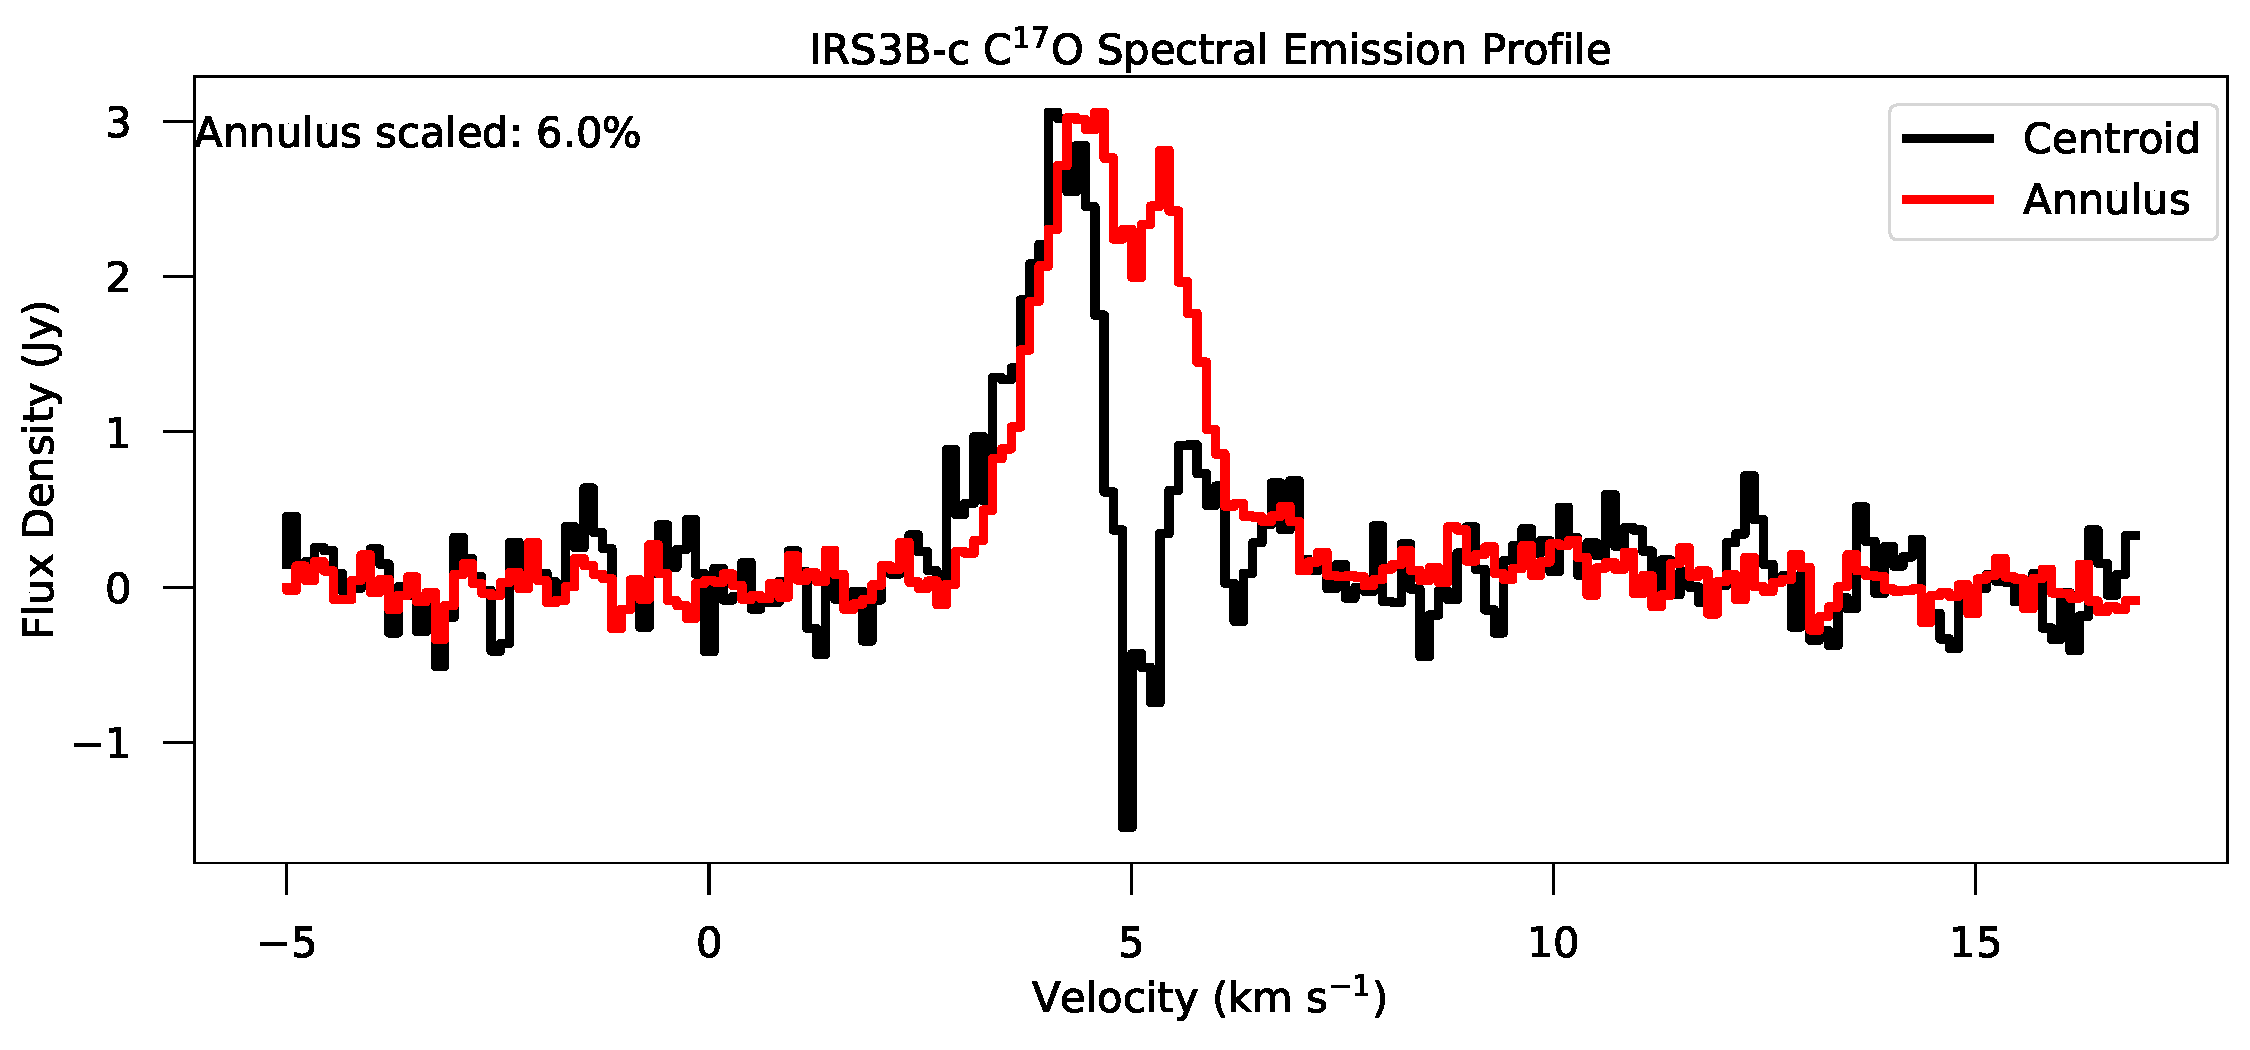
\includegraphics[width=\textwidth]{img/c17o-spectra-irs3b-c.pdf}
   \end{center}
   \caption{\cso\space integrated spectral emission profile of IRS3B-c, set to the rest frequency of \cso. The profiles were extracted by integrating the emission within an annulus, where the co-center of the annuli is set to the center point of IRS3B-c, while the inclination and position angle of the annuli is set to the IRS3B-ab parameters. The ``black'' profile is extracted from a central ellipse 2 times the size of the restoring beam, while the ``red'' profile is extracted from an annulus with the same width as the average restoring beam, three beam widths off of the source. The central emission features a deficit of emission towards line center. The profiles are normalized to highlight the emission profiles rather than the actual values of the emission.}\label{fig:irs3bspec}
\end{figure}
\begin{figure}[H]
  \begin{center}
   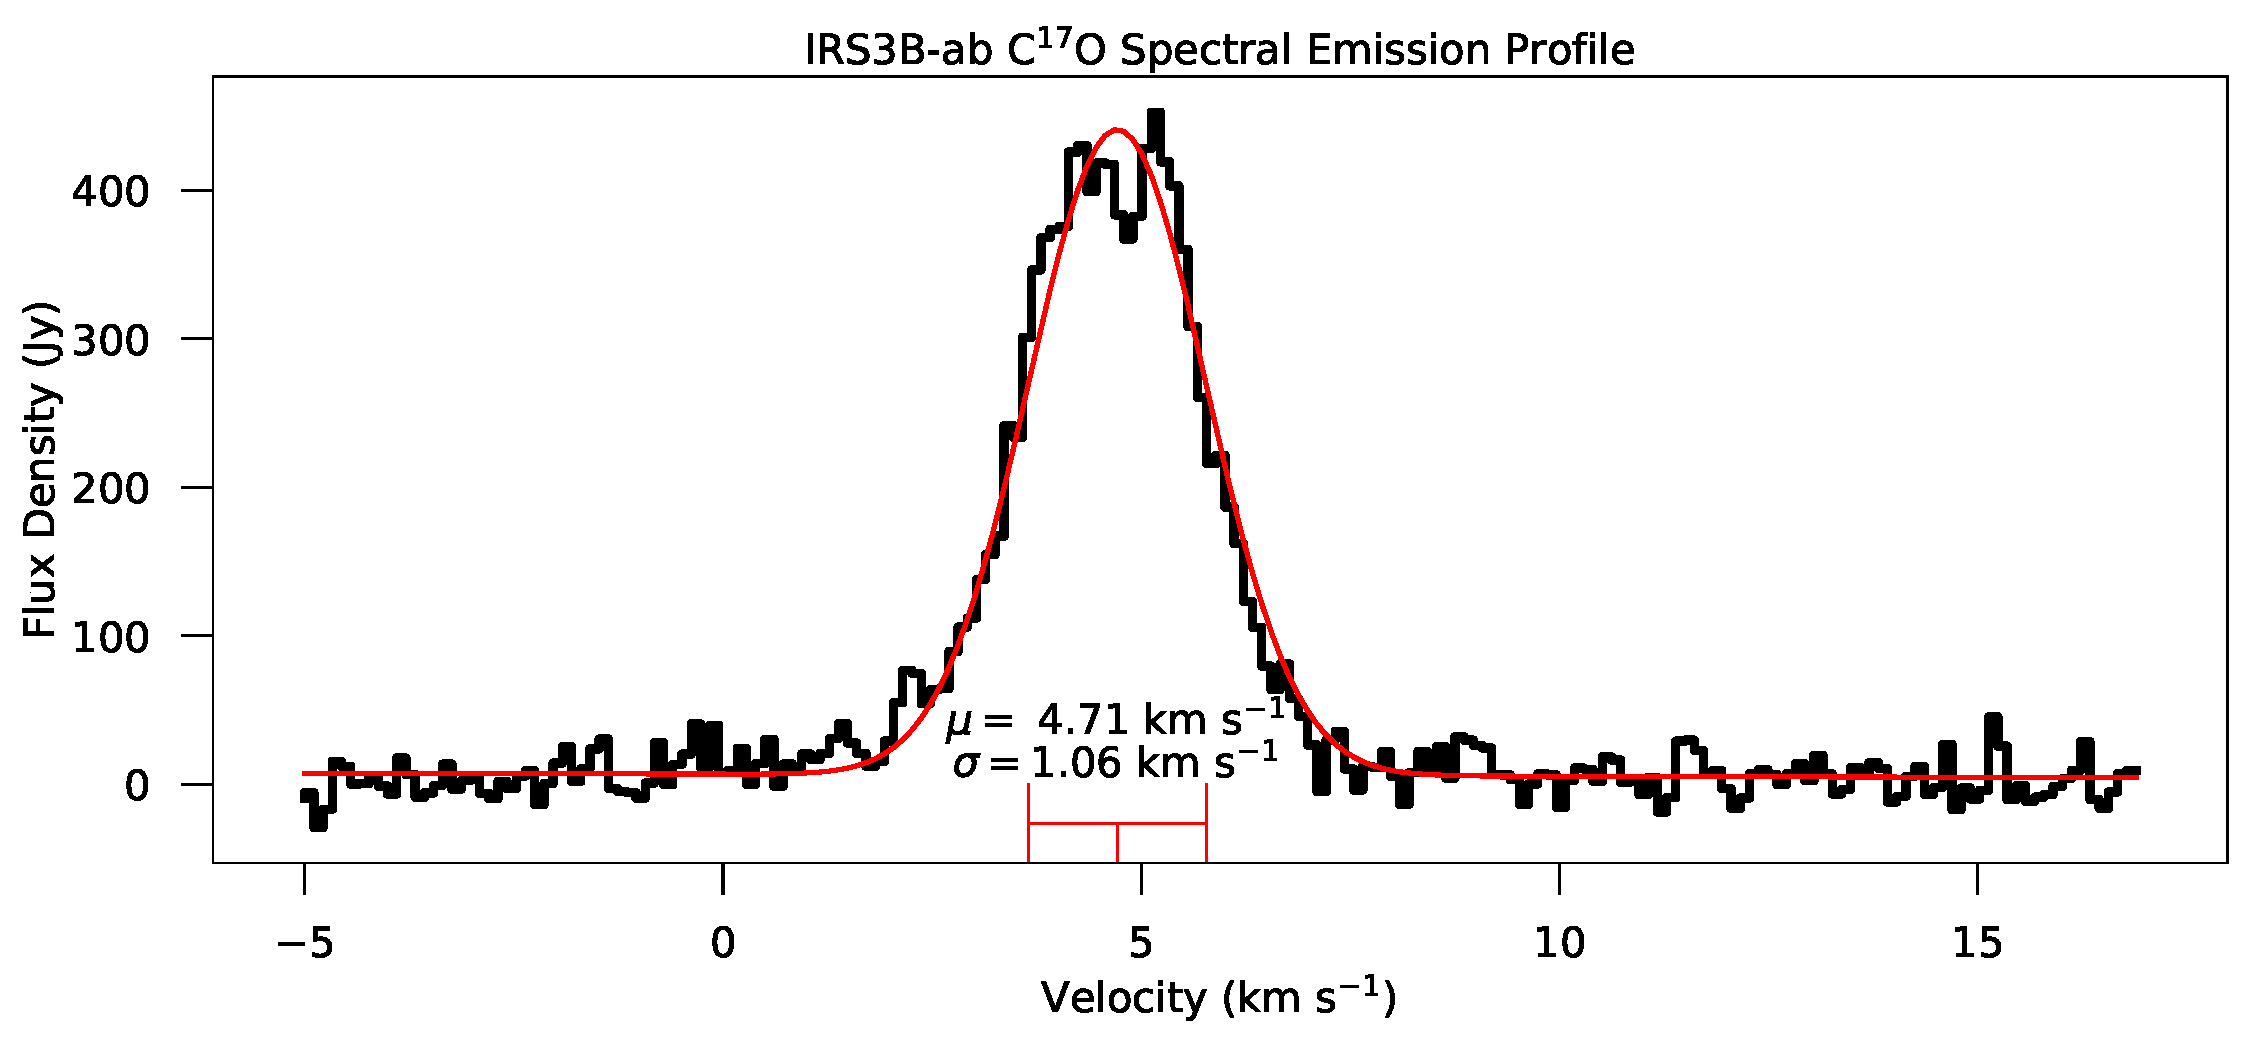
\includegraphics[width=\textwidth]{img/c17o-spectra-irs3b-ab.pdf}
   \end{center}
   \caption{\cso\space integrated spectral emission profile of IRS3B-ab, set to the rest frequency of \cso. The profile is extracted by integrating the emission within an ellipse, where the center, inclination, and position angle are set to the center point of IRS3B-ab. The ``black'' profile is extracted from a central ellipse the same size as the gaseous disk in Table~\ref{table:obssummary3}. The red line is a Gaussian fit to the spectra, with parameters $\mu=$4.71$^{+0.02}_{-0.02}$~\kms\space and $\sigma=$1.06$^{+0.02}_{-0.02}$~\kms.}\label{fig:irs3babspec}
\end{figure}
\begin{figure}[H]
  \begin{center}
   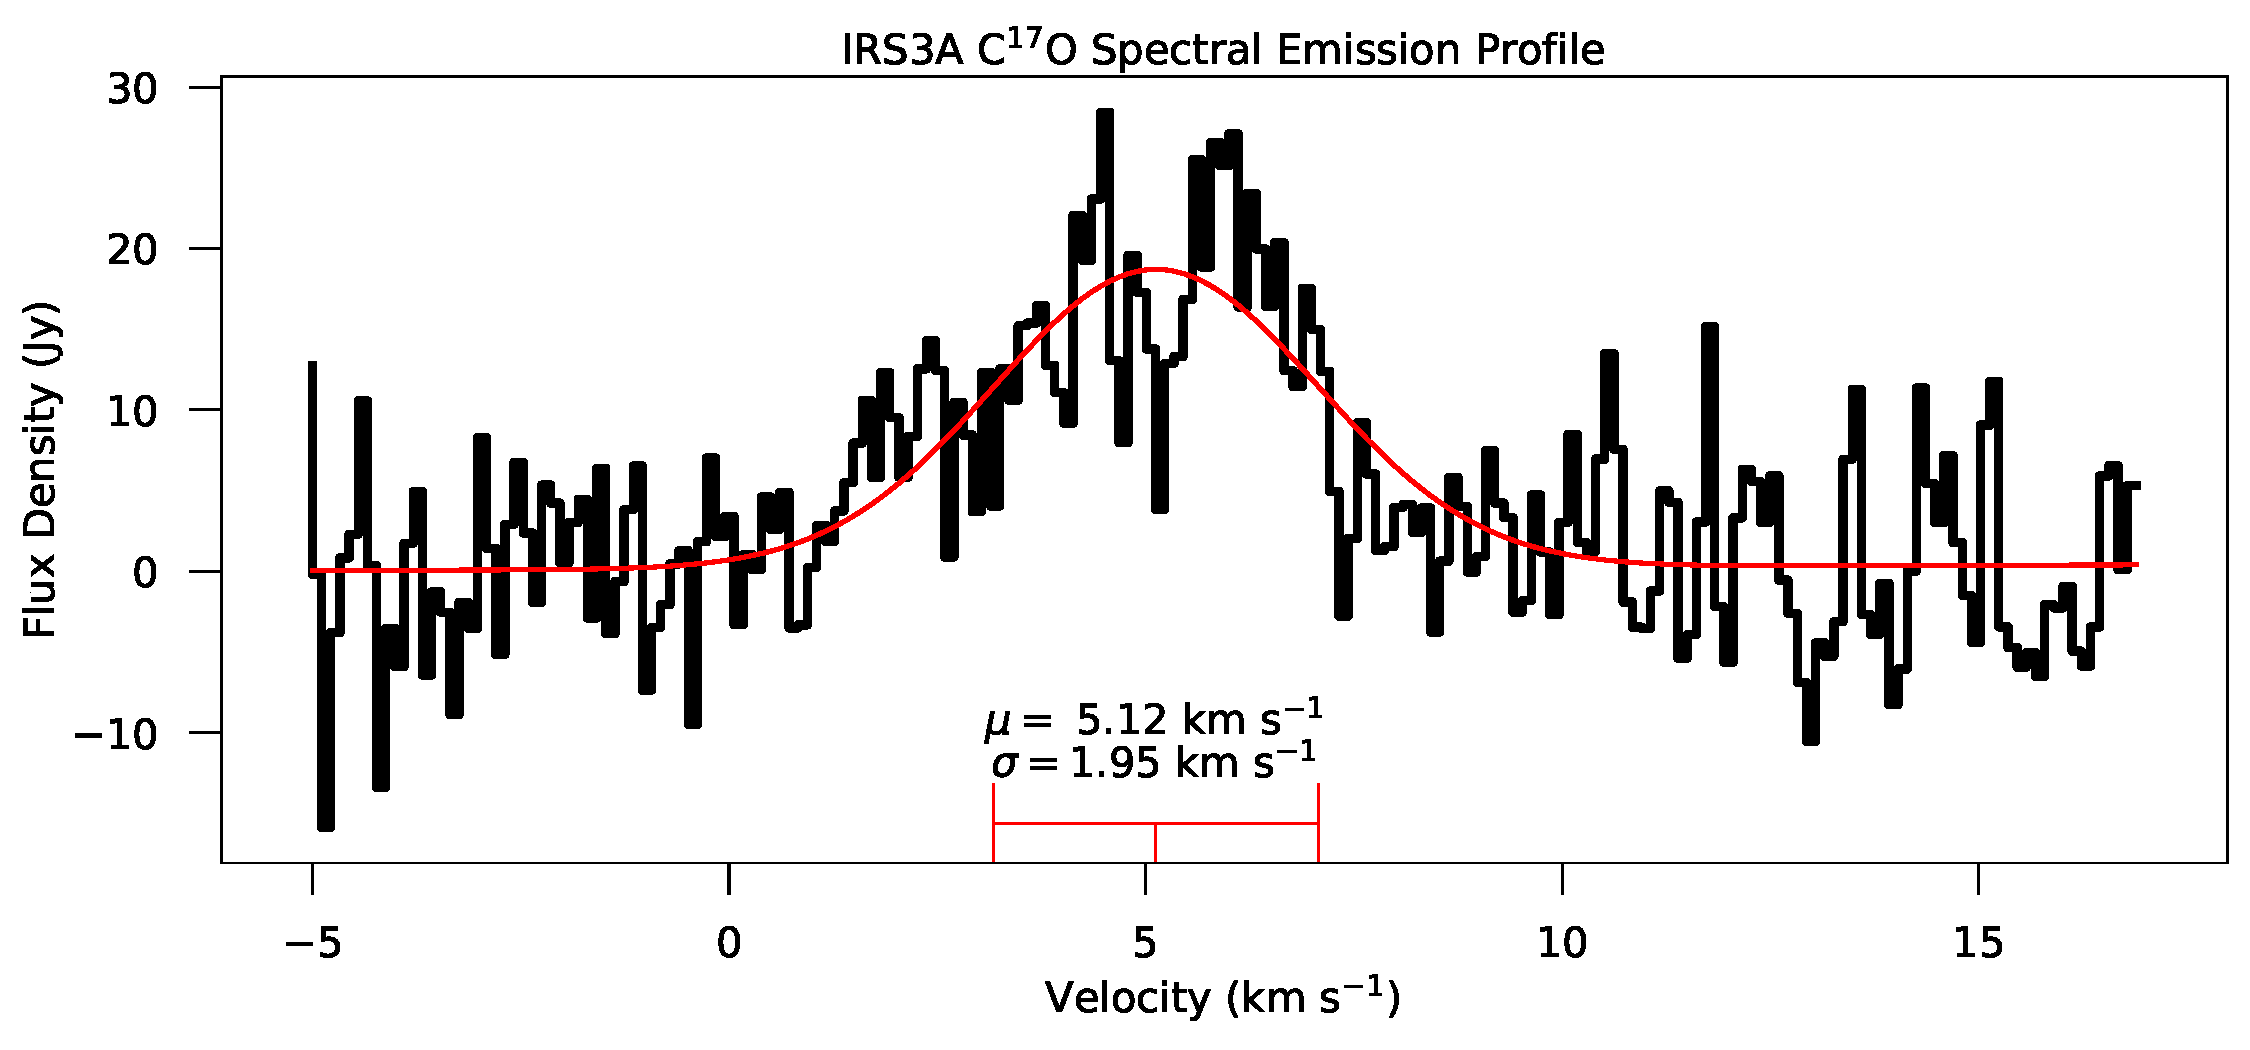
\includegraphics[width=\textwidth]{img/c17o-spectra-irs3a.pdf}
   \end{center}
   \caption{\cso\space integrated spectral emission profile of IRS3A, set to the rest frequency of \cso. The profiles were extracted by integrating the emission within an ellipse, where the center, inclination, and position angle are set to the center point of IRS3A. The ``black'' profile is extracted from a central ellipse the same size as the gaseous disk in Table~\ref{table:obssummary3}. The \cso\space emission towards this source is fainter than the emission from other dense gas tracers, thought to trace disk kinematics like that of \htcn.  The red line is a Gaussian fit to the spectra, with parameters $\mu=$5.12$^{+0.15}_{-0.15}$~\kms\space and $\sigma=$1.95$^{+0.75}_{-0.17}$~\kms.}\label{fig:irs3aspec}
\end{figure}

\section{Tertiary Subtraction and Gaussian Fitting}\label{sec:tertsub}
The continuum emission of the bright, embedded source, IRS3B-c, biases the analysis of the radial disk structure and circumstellar disk mass estimate of the IRS3B system. By removing this source, we can independently examine the disk and the tertiary source in order to characterize their properties separately~(Figure~\ref{fig:subclump}). In order to remove the tertiary source, we fit two Gaussians with a zero-level offset to the position of the source using the \textit{imfit} task in CASA (a point source and single Gaussian did not provide adequate fit while preserving the underlying disk emission). The offset serves to preserve the emission from the underlying IRS3B-ab disk emission. We also restricted the imfit task to a 0\farcs8$\times$0\farcs7\space ellipse around the source such that the fit does not extend into the surrounding emission from the spiral arms. With these parameters generated from the imfit task, we then constructed a model image of the tertiary. We used the CASA task \textit{setjy} to Fourier transform the model image and fill the model column of the measurement set with the model visibility data. We then use the task \textit{uvsub} to subtract this model from the data, producing the residual visibilities without the tertiary. A tertiary subtracted image is generated from this residual dataset and shown in Figure~\ref{fig:subclump} along with the model of the tertiary used to construct this dataset. The masses generated from this fit is \ab0.07~\solm, as described in Section~\ref{sec:dcont} and provided in Table~\ref{table:pvtable}. We then are able to reconstruct and taper the resulting visibilities to smooth over the substructure of the disk, in order to better fit the circum-multiple disk. The image (Figure~\ref{fig:subclumptaper}) is fit with a 2-D Gaussian using the \textit{imfit} in CASA and the results of the fit are provided in Table~\ref{table:obssummary3}.

\begin{figure}[H]
  \begin{center}
   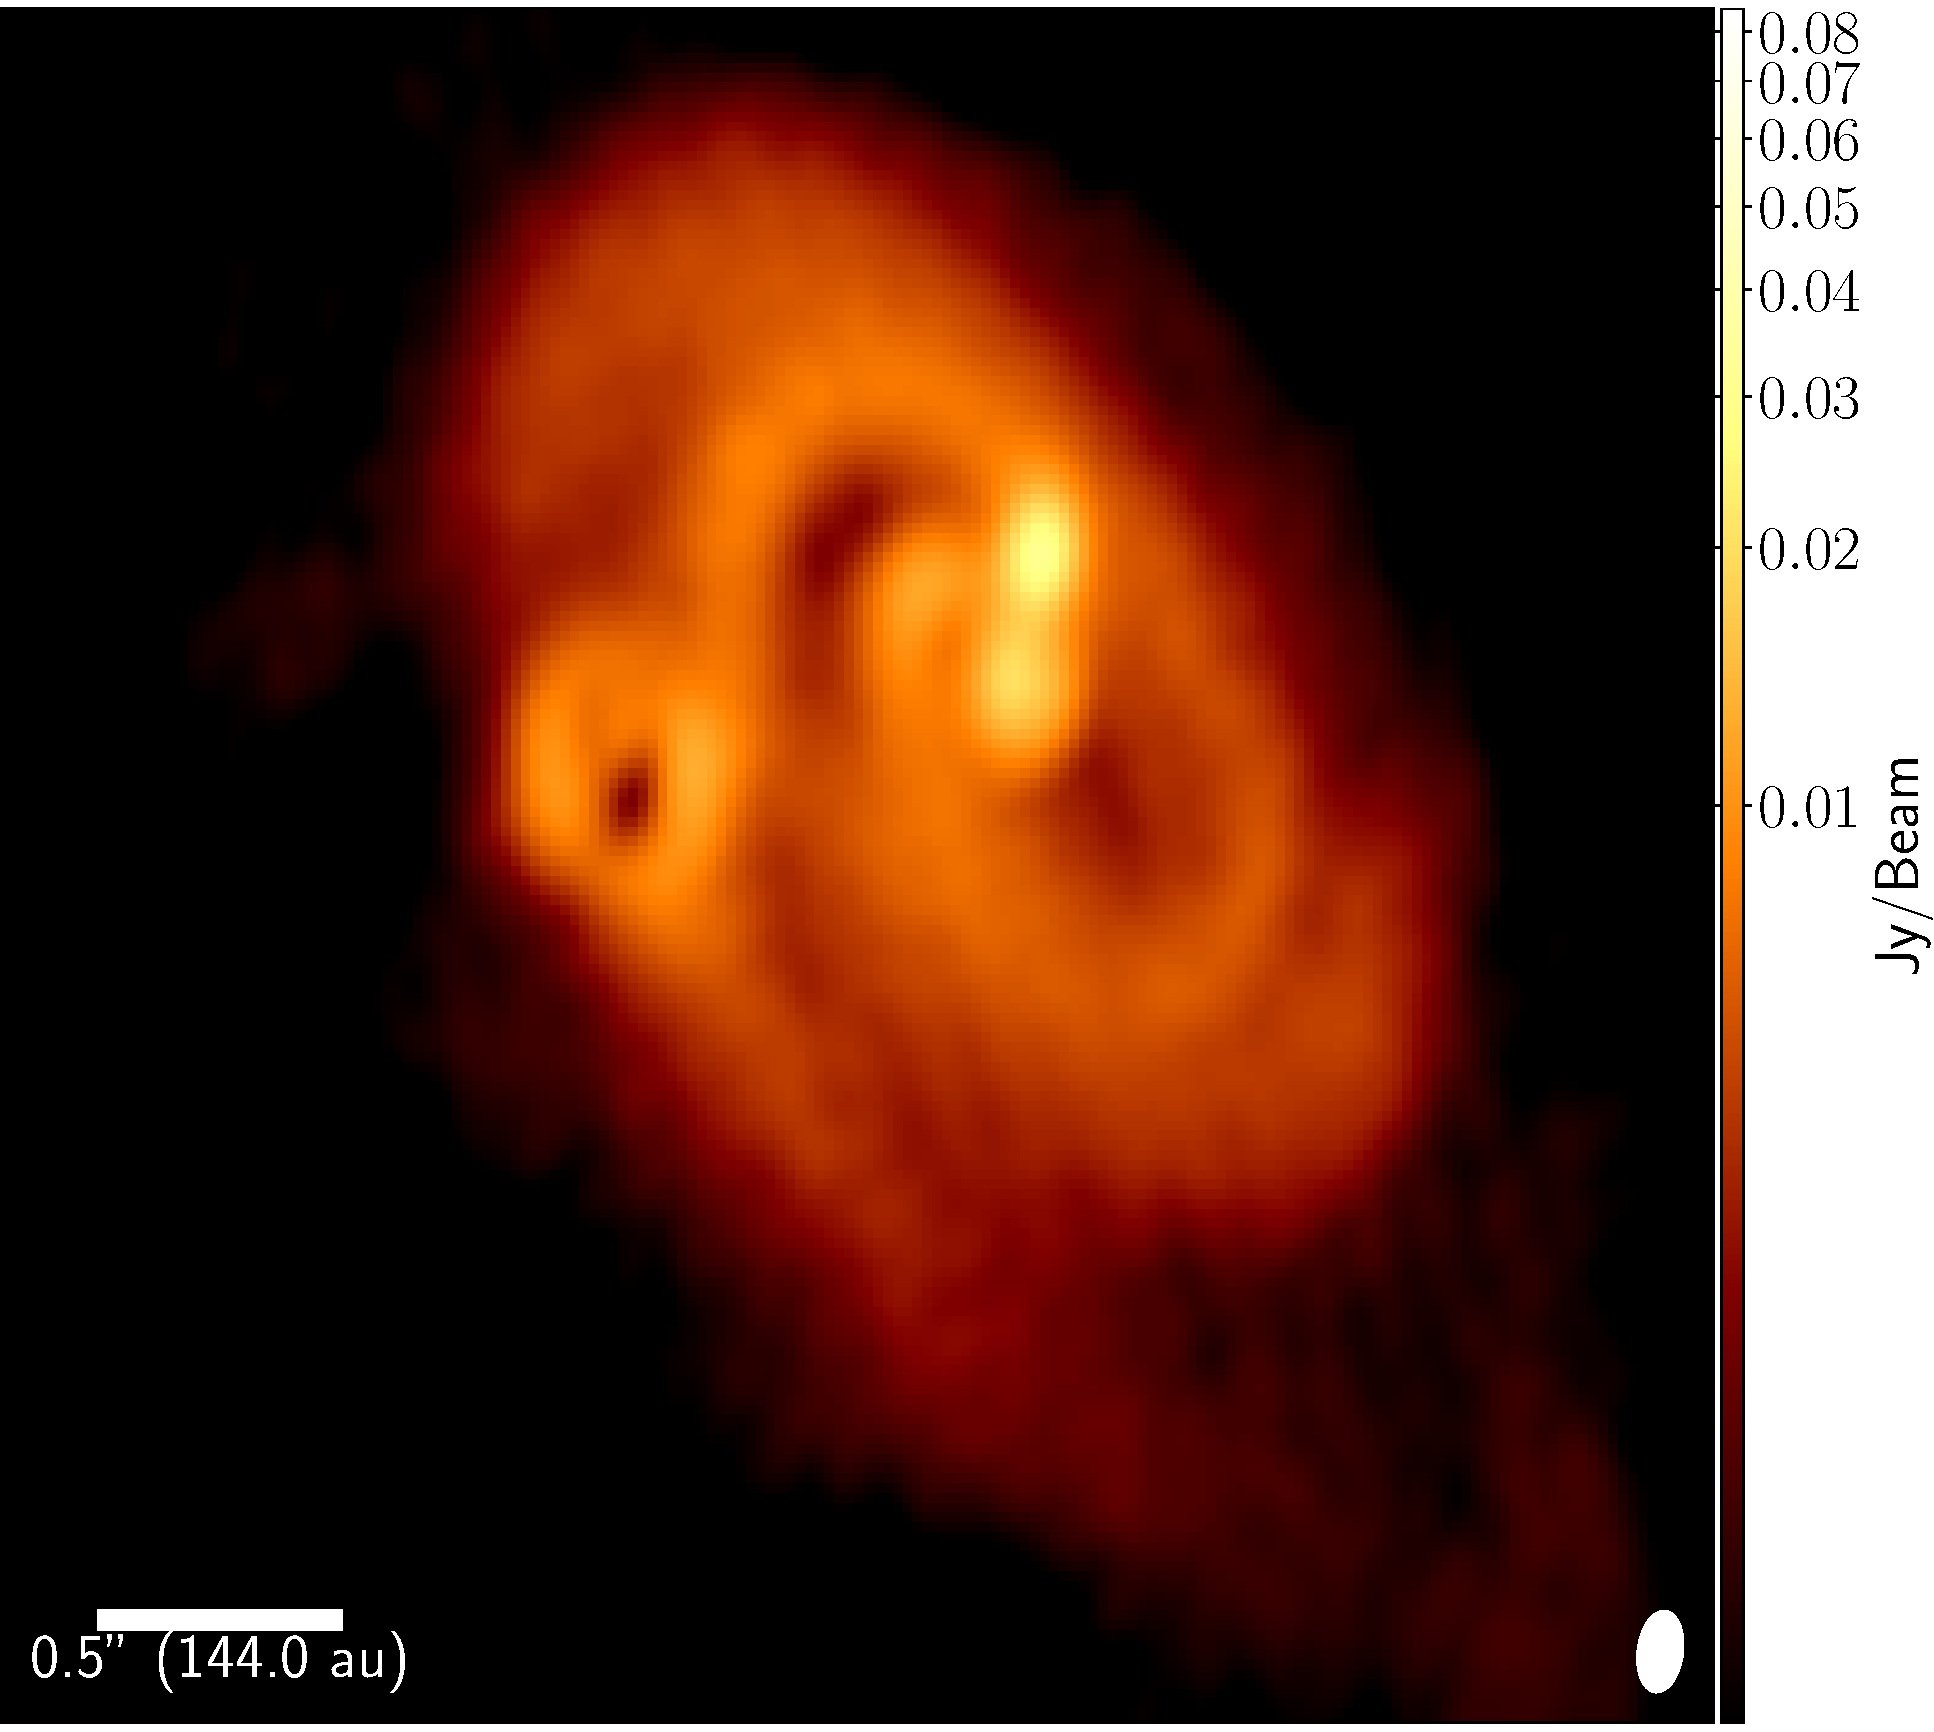
\includegraphics[width=0.48\textwidth]{img/L1448IRS3B-cont-subclump-robust05binary_uc.pdf} % co
   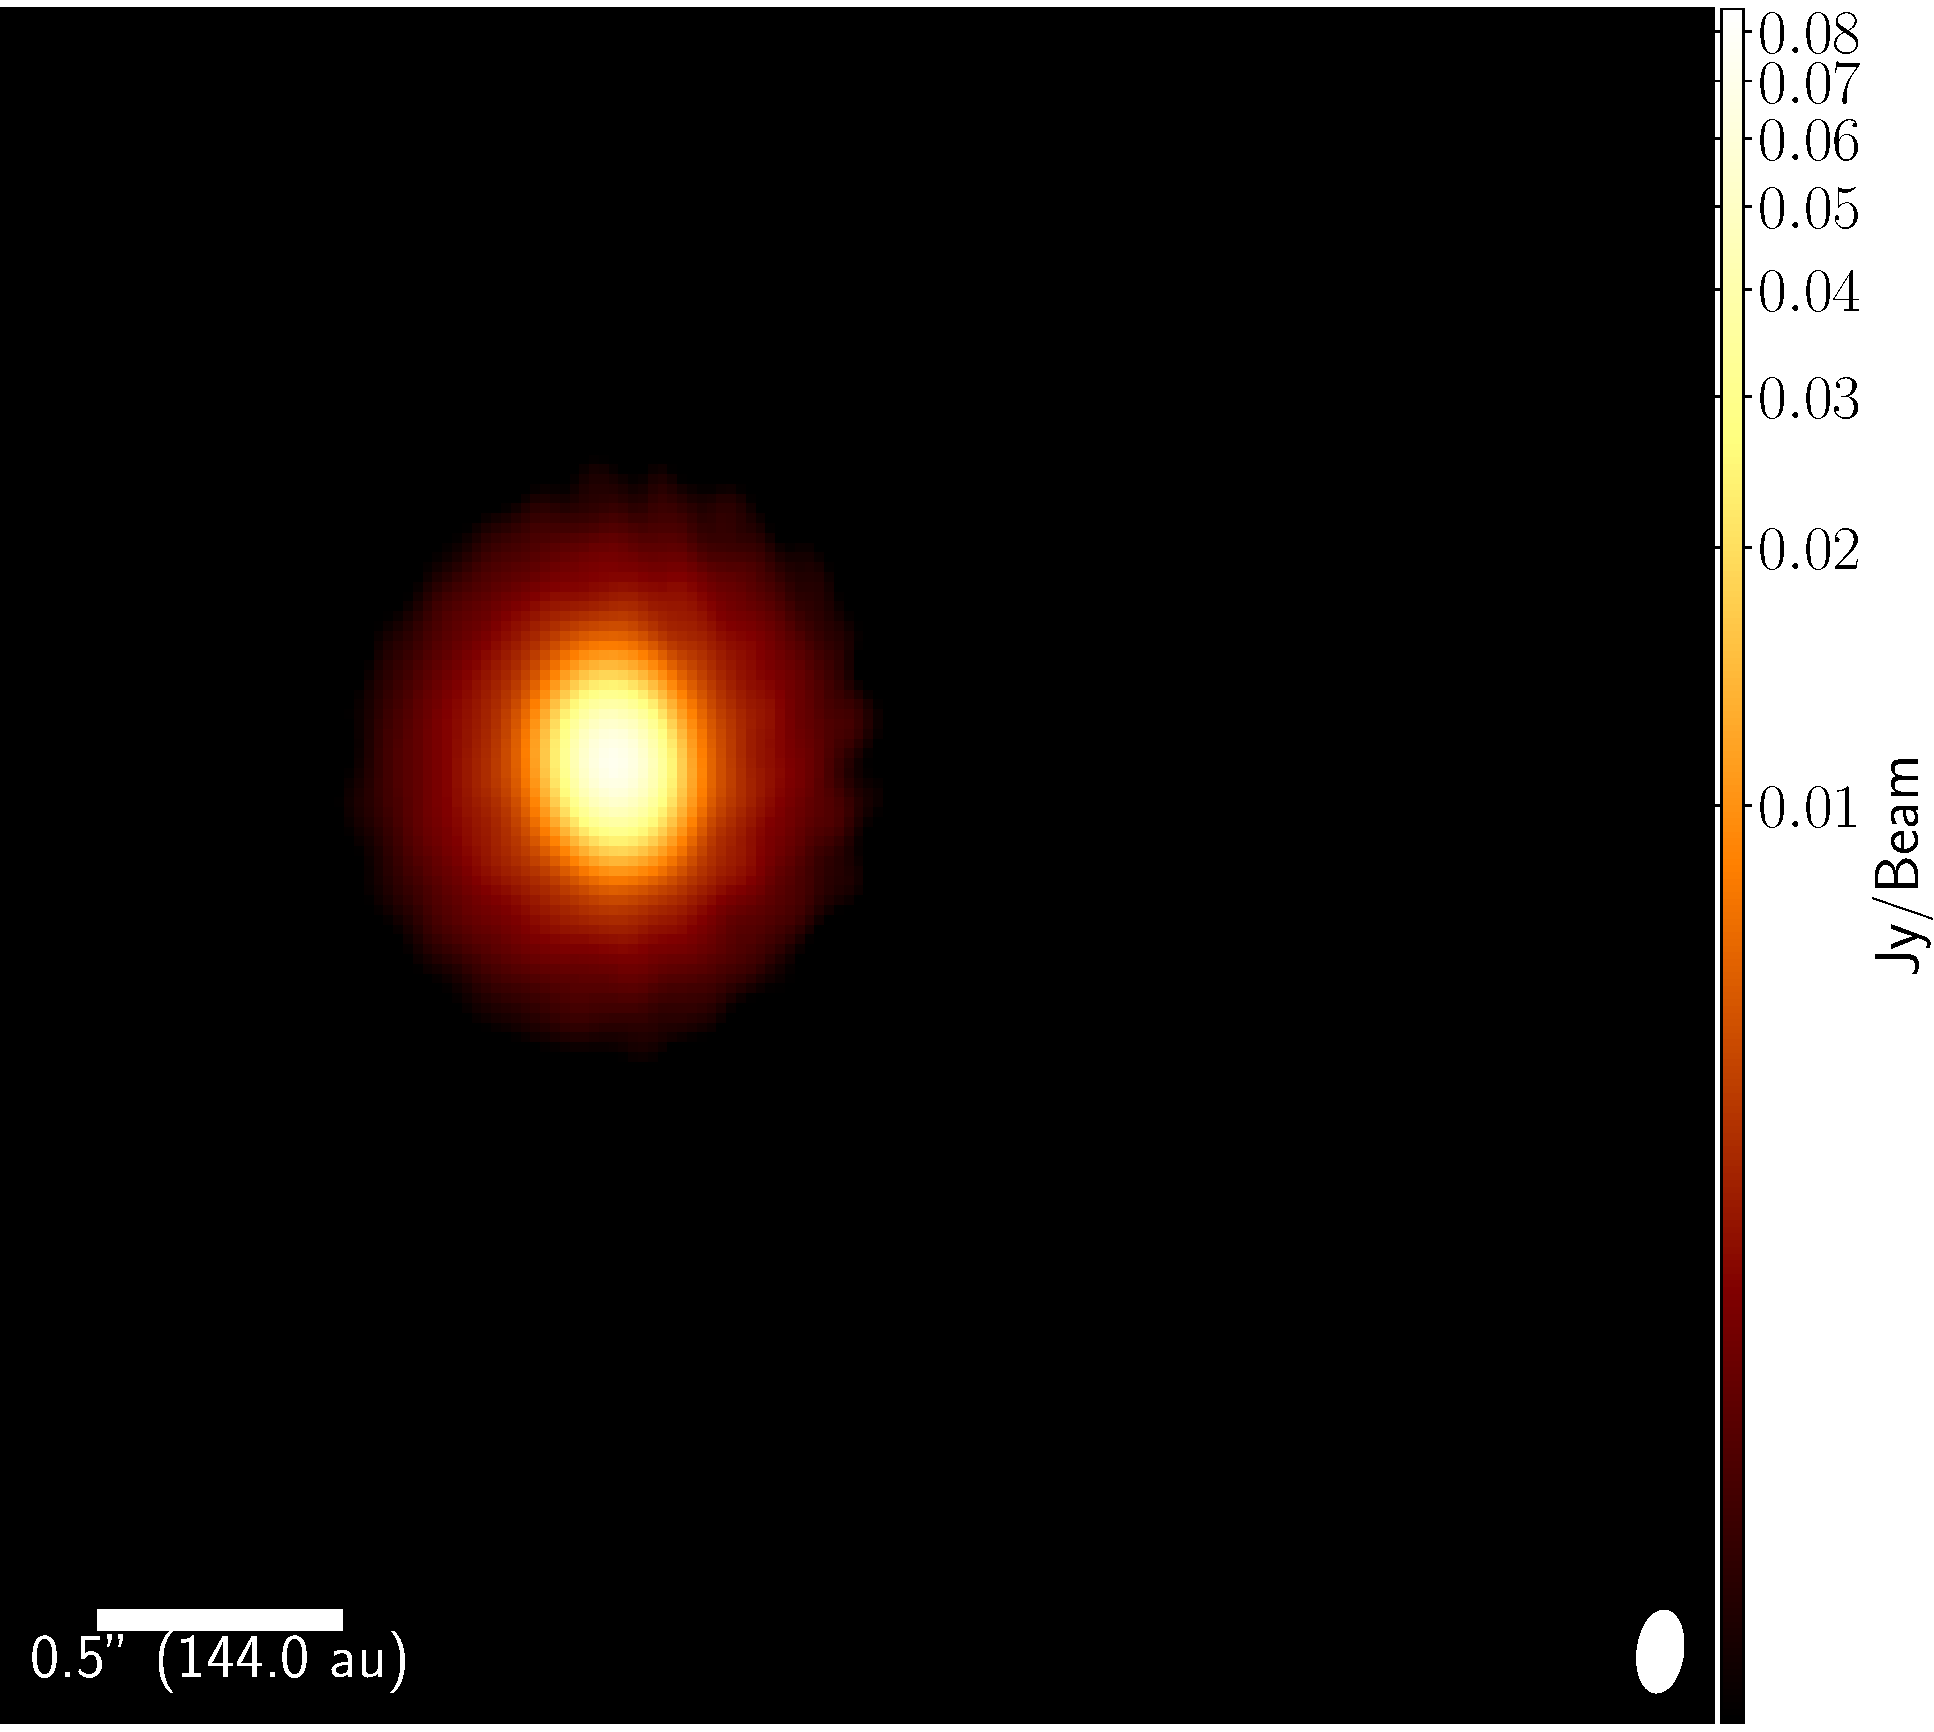
\includegraphics[width=0.48\textwidth]{img/tertiary-onlycont_uc.pdf} % co
   \end{center}
   \caption{Continuum (879~\micron) images of IRS3B with the tertiary clump removed (left image) for analysis and the model of the tertiary clump (right image). The tertiary model was constructed using two 2D Gaussians with a zero-level offset in order to properly restore the underlying disk emission without introducing additional features. The left image was used to exclude the embedded tertiary mass from the dust component of the circumstellar disk while the right image image was then used for analysis of the compact dust emission around the tertiary.} \label{fig:subclump}
\end{figure}

\begin{figure}[H]
  \begin{center}
   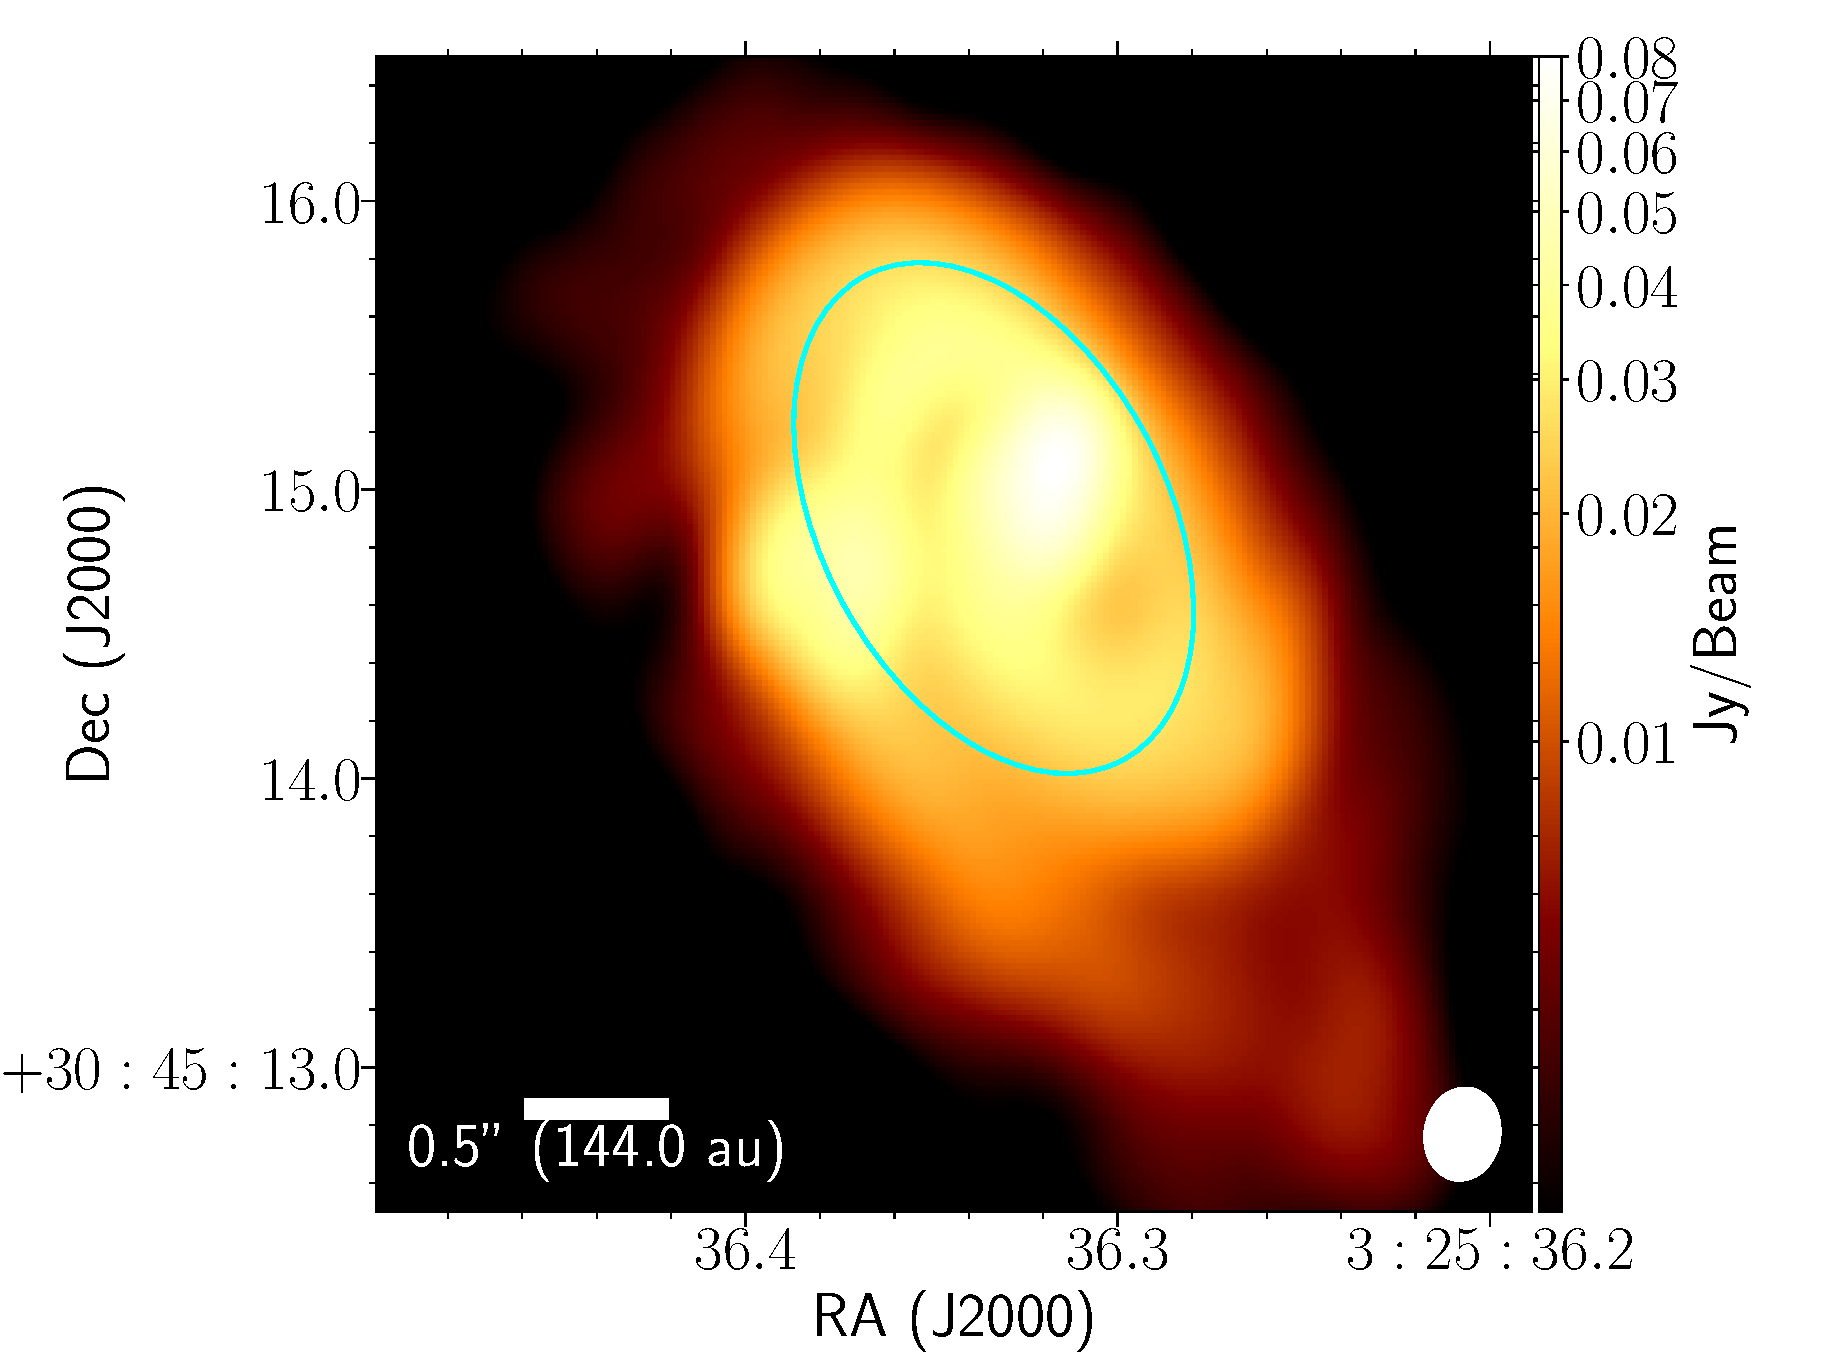
\includegraphics[width=0.48\textwidth]{img/L1448IRS3B-cont-subclump-robust2-uvtaper500taper500-remtert.pdf} % co
   \end{center}
   \caption{Continuum (879~\micron) image of IRS3B with the tertiary removed, reconstructed with Briggs weighing robust parameter of 2 and tapered to 500k$\lambda$. This smooths over the substructure of the continuum disk to enable fitting of the disk with a single 2-D Gaussian profile, without over-fitting the substructure. The cyan line is the Gaussian fit of the circum-multiple disk of IRS3B, with the major and minor axis of the ellipses defined by the FWHM major and minor axis of the 2-D Gaussian fit.} \label{fig:subclumptaper}
\end{figure}